\documentclass{article}

\usepackage{defines}

\usepackage{tikz}

\usepackage{caption}

\begin{document}

\tickettitle{1}{Понятия вектора, орта, сонаправленных векторов. Теорема о коллинеарности. Линейные операции над векторами (сумма, разность, произведение на число). Восемь свойств.}

\define{вектора}

Вектор --- направленный отрезок.

Вектор характеризуется:
\begin{enumerate}
	\item{}Длиной (модулем), $|\lvec{AB}|$, $|\vec{a}|$
	\item{}Направлением
\end{enumerate}

Нулевой вектор $\vec{0}$:
\begin{enumerate}
	\item{}$|\vec{0}|=0$
	\item{}Не имеет направления или направлен в любую сторону.
\end{enumerate}

\define{сонаправленных векторов}

\begin{minipage}{0.6\linewidth}
	Векторы $\vec{a}$ и $\vec{b}$ коллинеарны ($\vec{a}\parallel\vec{b}$), если они лежат на параллельных прямых. $(\forall \vec{a})\;\vec{a}\parallel\vec{0}$.

	Векторы $\vec{a}$ и $\vec{b}$ сонаправлены ($\vec{a}\upuparrows\vec{b}$), если:
	\begin{enumerate}
		\item{}$\vec{a}\parallel\vec{b}$ $\land$ они лежат по одну сторону от прямой, проходящей через их начала (\figref{1:codirectional}).
		\item{}Они лежат на одной прямой и направлены в одну сторону.
		\item{}$\vec{a}=\vec{0}\lor\vec{b}=\vec{0}$
	\end{enumerate}

	Векторы $\vec{a}$ и $\vec{b}$ противоположно направлены ($\vec{a}\updownarrows\vec{b}$), если $\vec{a}\parallel\vec{b}\land\lnot(\vec{a}\upuparrows\vec{b})$

\end{minipage}%
\begin{minipage}{0.4\linewidth}
	\centering
	\begin{tikzpicture}
		\draw (0,0)--(3,4);
		\draw (3,0)--(6,4);
		\draw (-0.75,0.6)--(6,2.4);
		\draw [-latex, thick] (4.5,2)--(5.25,3) node[midway, above left] {$\vec{a}$};
		\draw [-latex, thick] (0.75,1)--(1.5,2) node[midway, above left] {$\vec{b}$};
	\end{tikzpicture}
	\captionof{figure}{Сонаправленные векторы}\label{1:codirectional}
\end{minipage}

\define{равенства векторов}
\begin{align*}
	\vec{a}=\vec{b}\Lrarr |\vec{a}|=|\vec{b}|\land \vec{a}\upuparrows\vec{b}
\end{align*}

\define{орта}
\begin{align*}
	\vec{b}=\ort\vec{a}\Lrarr |\vec{a}|=1\land\vec{a}\upuparrows\vec{b}
\end{align*}

$\vec{e}_a=\ort\vec{a}$ --- нормированный вектор $\vec{a}$.

\pagebreak

\sectitle{Линейные операции над векторами}

\define{сложения векторов, свойства 1-4}

\begin{minipage}{0.6\linewidth}
	Суммой векторов $\vec{a}$ и $\vec{b}$ ($\vec{a}+\vec{b}$), следующих друг\\
	за другом называется вектор от начала первого\\
	до конца последнего (\figref{1:sum}).

	Свойста сложения векторов:
	\begin{enumerate}
		\item{}Коммутативность: $\vec{a}+\vec{b}=\vec{b}+\vec{a}$ (Доказывается через свойства параллелограмма на \figref{1:sum})
		\item{}Ассоциативность: $(\vec{a}+\vec{b})+\vec{c}=\vec{a}+(\vec{b}+\vec{c})$ (Следует из определения)
		\item{}Нейтральный элемент: $\vec{a}+\vec{0}=\vec{a}$
		\item{}Обратный элемент: $(\forall \vec{a})\;\exists\vec{b}:\vec{a}+\vec{b}=\vec{0}$
	\end{enumerate}
\end{minipage}%
\begin{minipage}{0.4\linewidth}
	\centering
	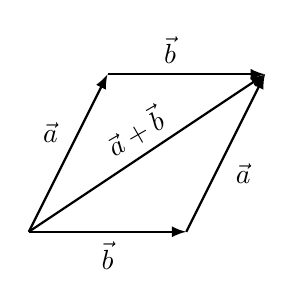
\begin{tikzpicture}
		\draw [-latex, thick] (0,0)--(1,2) node[midway, above left] {$\vec{a}$};
		\draw [-latex, thick] (1,2)--(3,2) node[midway, above left] {$\vec{b}$};
		\draw [-latex, thick] (0,0)--(2,0) node[midway, below] {$\vec{b}$};
		\draw [-latex, thick] (2,0)--(3,2) node[midway, below right] {$\vec{a}$};
		\draw [-latex, thick] (0,0)--(3,2) node[midway, above, rotate=30] {$\vec{a}+\vec{b}$};
	\end{tikzpicture}
	\captionof{figure}{Коммутативность сложения}\label{1:sum}
\end{minipage}

\define{разности векторов}

Разностью $\vec{a}$ и $\vec{b}$ ($\vec{a}-\vec{b}$) называется $\vec{c}$: $\vec{a}=\vec{b}+\vec{c}$. Существование такого вектора обеспечивается четвёртым свойством сложения:
$\vec{c}=(-\vec{b})+\vec{a}$, где $(-\vec{b})$ --- обратный элемент к $\vec{b}$.

\define{произведения вектора на число, свойства 5-8}

Произведением $\vec{a}$ на $\gamma\in\R$ называется $\vec{p}=\gamma\vec{a}$:
\begin{align*}
	 & |\vec{p}|=|\gamma||\vec{a}| &  & \land &  &
	\begin{cases}
		\vec{p}=\vec{0}             & \text{при $\gamma=0$} \\
		\vec{p}\upuparrows\vec{a}   & \text{при $\gamma>0$} \\
		\vec{p}\updownarrows\vec{a} & \text{при $\gamma<0$}
	\end{cases}
\end{align*}
$\vec{e}_a=\ort\vec{a}=\cfrac{\vec{a}}{|\vec{a}|}$

Свойства произведения вектора на число:
\begin{enumerate}
	\setcounter{enumi}{4}
	\item{}Ассоциативность относительного числового сомножителя: $\alpha(\beta\vec{a})=(\alpha\beta)\vec{a}$
	\item{}Дистрибутивность векторного сомножителя: $(\alpha+\beta)\vec{a}=\alpha\vec{a}+\beta\vec{a}$
	\item{}Дистрибутивность числового сомножителя: $\alpha(\vec{a}+\vec{b})=\alpha\vec{a}+\alpha\vec{b}$
	\item{}Произведение на 1: $1\cdot\vec{a}=\vec{a}$
\end{enumerate}

\pagebreak

\theorem
\begin{align*}
	\vec{a}\neq \vec{0}\land \vec{a}\parallel\vec{b}\Lrarr \exists!\alpha\in\R:\vec{b}=\alpha\vec{a}
\end{align*}

\onlyif

Пусть $\vec{b}=\alpha\vec{a}$. Покажем, что такой $\alpha$ едиственный, найдя его представление с помощью эквивалентных преобразований.
\begin{align*}
	\vec{b}=\alpha\vec{a}\Lrarr
	\begin{cases}
		|\vec{b}|=|\alpha||\vec{a}| \\
		\vec{b}\upuparrows\alpha\vec{a}
	\end{cases}\Lrarr
	\begin{cases}
		|\alpha|=\cfrac{|\vec{b}|}{|\vec{a}|}              \\
		\alpha>0 & \text{при } \vec{b}\upuparrows\vec{a}   \\
		\alpha<0 & \text{при } \vec{b}\updownarrows\vec{a} \\
		\alpha=0 & \text{при }\vec{b}=\vec{0}
	\end{cases}
\end{align*}

Одно из условий $\vec{b}\upuparrows\vec{a}$, $\vec{b}\updownarrows\vec{a}$ или $\vec{b}=\vec{0}$ соблюдается, тк $\vec{a}\parallel\vec{b}$.

\enough

По определениям произведения вектора на число и равенства векторов:
\begin{align*}
	\vec{b}=\alpha\vec{a}\Rarr(\vec{b}\parallel\alpha\vec{a})\land(\alpha\vec{a}\parallel\vec{a})\Rarr\vec{a}\parallel\vec{b}
\end{align*}

Расммотрим случай $\vec{a}=\vec{0}$:
\begin{align*}
	\vec{a}=\vec{0}\Rarr
	\begin{cases}
		\vec{a}=\vec{b}=\vec{0} \\
		\vec{b}=\alpha\vec{a}
	\end{cases}\Rarr (\forall \alpha\in\R)\;\vec{b}=\alpha\vec{a}
\end{align*}

Таким образом, из $\vec{a}=\vec{0}$ следует не единственность $\alpha$, тогда из единственности $\alpha$\\
будет следовать $\vec{a}\neq\vec{0}$.

Таким образом:
\begin{align*}
	\exists!\alpha\in\R:\vec{b}=\alpha\vec{a}\Rarr\vec{a}\neq\vec{0}\land\vec{a}\parallel\vec{b}\qed
\end{align*}


\end{document}
